%!TEX root = ../thesis.tex
%*******************************************************************************
%*********************************** First Chapter *****************************
%*******************************************************************************

\chapter{Discussion}  %Title of the First Chapter

\ifpdf
    \graphicspath{{Chapter7/Figs/Raster/}{Chapter7/Figs/PDF/}{Chapter7/Figs/}}
\else
    \graphicspath{{Chapter7/Figs/Vector/}{Chapter7/Figs/}}
\fi


%********************************** %First Section  **************************************
\section{Converting iPG into Blood Flow for detecting venous and arterial changes} %Section - 7.1 
\label{section discussion 1}
As it has been discussed in this document, there are two ways to calculate blood flow from the iPG data. Initially, it is needed to model the segment of the body as a cylinder. Luckily, most of the body parts can be expressed as this geometrical figure. For this study, a device was designed to measure the change of volume in the forearm. Eventually, this could be calibrated to work in other parts of the body such as lower extremities. 

The study performed in this document seeks to demonstrate how the iPG data could help to detect changes in venous and arterial circulation. According to the literature, iPG is a method used to quantify blood flow from the principle that the impedance of a body part is directly proportional to its volume as described by Nyober's equation  (see equation \ref{eq:Nyober}).  Hence, since the 1970's this theory has been tested assuring the effectiveness of the method. 

There are different contributors to the impedimetric signal. One of them are the tissues such as fat, muscle, blood and bone. Most of this organs have intrinsic impedances when its movement is limited because motion changes different variables that could affect their impedance values. The sum of all these resistive values is known as basal impedance.  However,  the circulatory system is dynamic and create small changes during the cardiac cycle.  When the ventricles contract, it produces a slight increase in the size of the vessels by filling them with blood.
\mynote{check a reference about circulatory and added to this section. Also, check how to related to the medical background}. Therefore, this filling of blood within the tissue raises its total volume. Hence, knowing the rate of change of volume in time can be translated into the flow rate.

The first method to measure blood flow is called venous occlusion plethysmography \cite{wilkinson2001venous}. This approach inquires the increment of impedance when an occlusion is performed in the upper part of a limb using an inflatable cuff. The most common occlusion level is about \SI{40}{\mmHg} for a determined time. This occlusion could be for some seconds until minutes depending on the study to be done. 

By occluding the venous return and not altering the arterial flow, blood can enter into the limb but cannot leave.  As a result, there is a linear increase in the volume of the limb. Hence, this gain of capacity can be quantified by the impedimetric method which is clearly perceptible in the variation of the basal impedance. In fact, this is because the blood begins to cluster in the limb. As the blood's population increases, the conductivity of the forearm's section also rises in volume. Therefore, the resistivity proportionally decreases. 

During the experiment presented in this document the venous occlusion occurred throughout region 1 and region 2.  As shown by figure \ref{fig:rb:all_participants}, it is clear that most of the participants experience a variation in their basal impedance readings.  However, some of them were affected by motion which produced changes in the trend, like in participant 1. However, in most of the participants there was a linear decrease of impedance. 

In a similar situation, there was a reduction in the forearm's inflow when the brachial artery in the upper arm was partially occluded at the midpoint of the participant's blood pressure. Performing this action stops the venous return but also alters the incoming arterial flow \mynote{Check a paper about changing the elasticity of a tube changes its flow}. As a result, again the forearm's volume increases shifting its resistivity. It was noticed that when this occurs, the basal impedance decreases in a larger slope. This greater slope might be an indication of a higher laminar flow coming from the artery \mynote{Check what happens during arterial occlusion}. This effect can be confirmed by the data obtained from the Doppler ultrasound. In figure \ref{fig:DU_flow} can be clearly seen that the participants experienced a decrease in their flow in the region 4 of the data between \SIrange{780}{960}{\second}.   

All along total occlusion (Region 6) seemed that there was not a clear change trend of the participant's basal impedance.  Because both arterial and venous flow were blocked, there was not blood flow of any kind in the arm section. Therefore, this is the real basal impedance where all the tissues with their blood content were measured. The DC components of the PPG signal had a similar behaviour to this event where all participants had different responses. Indeed, only the Doppler ultrasound signal was able to reproduce a biological zero, the rest of the instruments showed some level of noisy data. 

By quantifying the blood flow from the basal impedance signal can be seen that there was not a significant change in its average rate. The mean value in venous occlusion was equivalent to \flowbasalvenous{} which is quite similar to the calculated mean arterial that was \flowbasalarterial{}. From this, it can be concluded that just by estimating the blood flow from the impedimetric measurements is not possible to have a clear difference between either arterial or venous occlusion.

However, the iPG signal can provide additional information that could give a clue about the change of flow during the occlusive events. This oscillatory signal comes from the expansion of the arteries and venous during the heart cycle. The filling of blood within the segment being examined creates a tiny change in the impedance. In other words, the basal impedance also contains a dynamic component that varies with the circulation. This small part is just a fraction of the total signal. In fact, the contribution of this dynamic signal is just \SI{0.04}{\percent} to the total impedance. Hence, the device described in chapter \ref{chapter design} was able to isolate satisfactory this waveform and provide a high-resolution version of this signal.

Obtaining this level of detail was important as provided more features about changes in different parts of the impedance plethysmography waveform. The signal collected from this section of the arm gave characteristics of the circulatory process. Three points were clearly identified as shown in \ref{section results 3.1}. Nonetheless, this signal is unique to this set-up, waveforms from other devices have reported unlike waveform shape when used in different parts of the body \mynote{Look for papers showing plethysmographic waveform}. The plethysmographic waveform obtained contains information about the systolic peak, the dicrotic notch and the diastolic peak which were clearly identified by the algorithm implemented \mynote{I have to add a part where I explain how the algorithm works}. 


  

%********************************** %Second Section  *************************************
\section{How much is related the iPG blood flow with other instruments?} %Section - 7.2
\label{section discussion 4}

%********************************** % Third Section  *************************************
\section{Option to evaluate blood flow using iPG DC and AC waveforms}  %Section - 7.3 
\label{section discussion 3}


\begin{figure}[!htpb]
	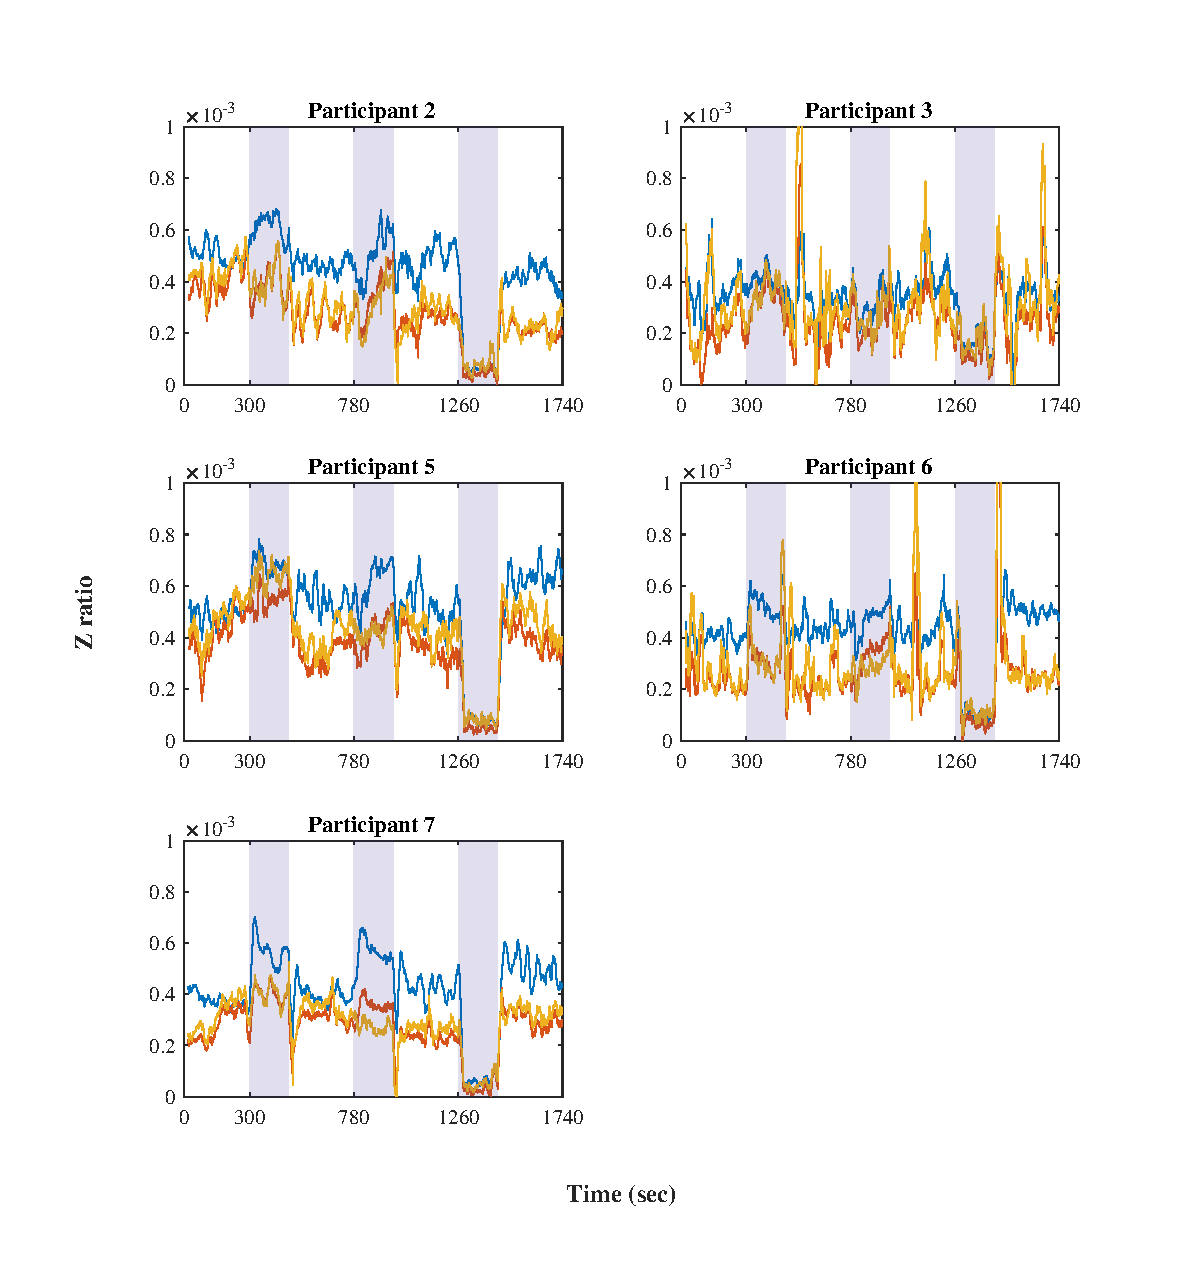
\includegraphics[width=1\textwidth,keepaspectratio]{figure1}    
	\caption[Bland and Altman plot of the relation between LDF and iPG]{Bland and Altman~\cite{bland1986statistical} plot of the relation between LDF and iPG. Data set corresponds to participants 2, 5, 6 and 7. The data has been normalised comparing the amplitude of both measurements. The different regions has been plotted with various colours and symbols to differentiate every event. The dotted line represents the perfect agreement, the dark line is the linear regression.}
	\label{fig:ratio Z}
\end{figure}

\begin{figure}[!htpb]
	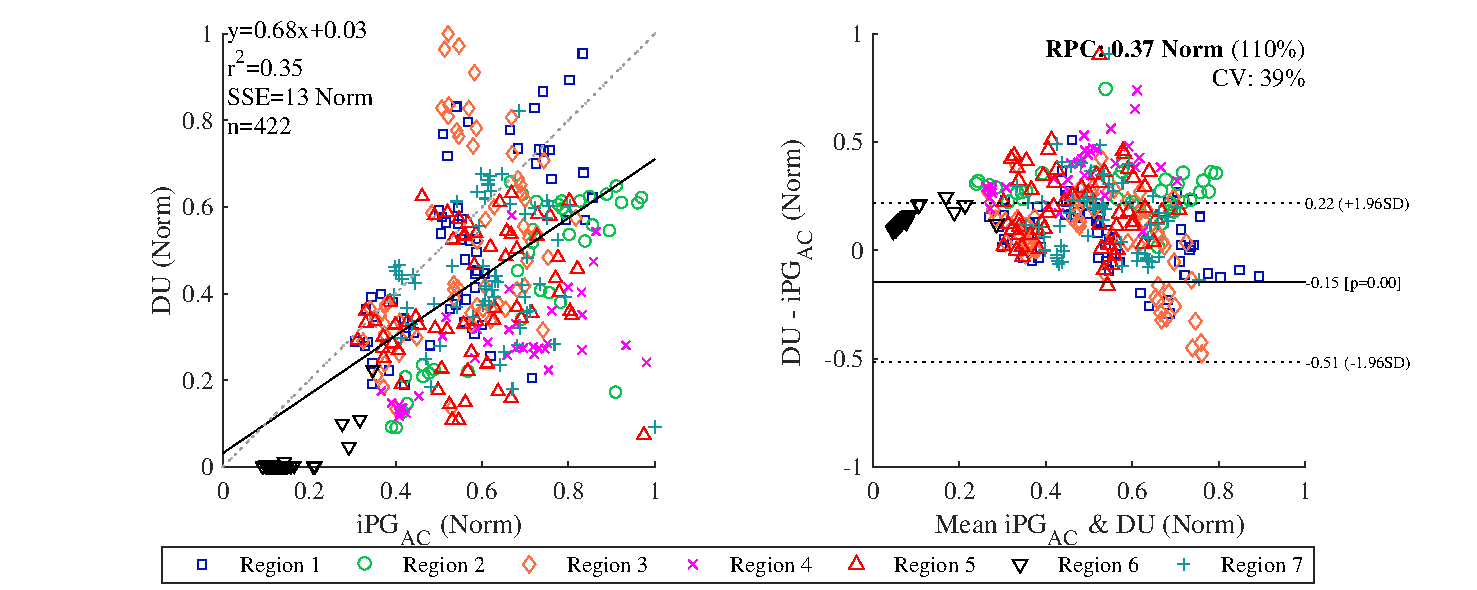
\includegraphics[width=1\textwidth,keepaspectratio]{figure2}    
	\caption[Bland and Altman plot of the relation between LDF and iPG]{Bland and Altman~\cite{bland1986statistical} plot of the relation between LDF and iPG. Data set corresponds to participants 2, 5, 6 and 7. The data has been normalised comparing the amplitude of both measurements. The different regions has been plotted with various colours and symbols to differentiate every event. The dotted line represents the perfect agreement, the dark line is the linear regression.}
	\label{fig:ration Z bar}
\end{figure}
